\EXERCISE
$8$
 مهره رنگی با 
$8$
  رنگ متفاوت 
$A, B, C, D, E, F, G, H$
در اختیار داریم و می‌خواهیم این مهره‌ها را در جایگاه‌های مشخص شده دور مربع قرار دهیم.
    \begin{center}
     	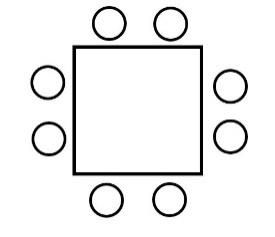
\includegraphics[scale=0.2]{./1.png}
    \end{center}
الف) چند حالت برای گذاشتن مهره‌ها دور مربع وجود دارد؟(دقت کنید جایگشتی که حاصل دوران دیگری است را دو بار نشمارید: مثلا شکل‌های (a) و (b) یکسان هستند ولی (a) و (c) یکسان نیستند.)
\begin{center}
	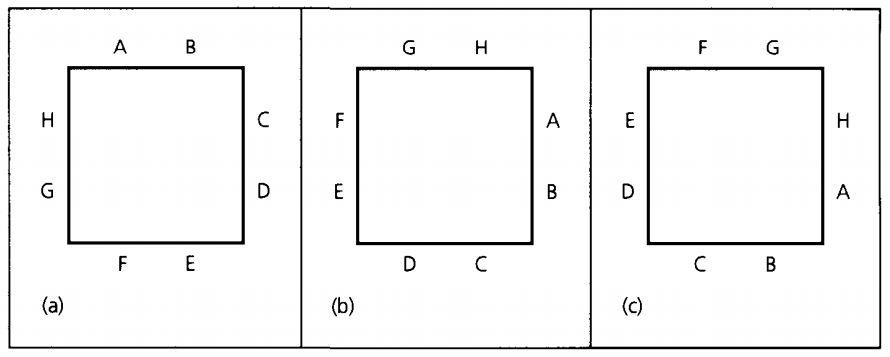
\includegraphics[scale=0.3]{./2.png}
\end{center}
ب) چند حالت چینش وجود دارد که در آن‌ها دو رنگ A و B به هیچ شکلی کنار هم نباشند؟